\documentclass[aspectratio=169]{beamer}

\usetheme{Madrid}
\usecolortheme{seahorse}
\usefonttheme{professionalfonts}

\usepackage{listings}
\usepackage{xcolor}
\usepackage{tikz}
\usepackage{booktabs}
\usepackage{hyperref}
\usepackage{textcomp}
\usepackage{microtype}

\definecolor{codebg}{HTML}{1E1E2E}
\definecolor{codegreen}{HTML}{A6E3A1}
\definecolor{codeblue}{HTML}{89DCEB}
\definecolor{codeyellow}{HTML}{F9E2AF}
\definecolor{codegray}{HTML}{6C7086}
\definecolor{codepurple}{HTML}{CBA6F7}
\definecolor{codeorange}{HTML}{FAB387}
\definecolor{codewhite}{HTML}{CDD6F4}

\lstdefinestyle{clang}{
  backgroundcolor=\color{codebg},
  basicstyle=\ttfamily\footnotesize\color{codewhite},
  keywordstyle=\color{codepurple}\bfseries,
  commentstyle=\color{codegray}\itshape,
  stringstyle=\color{codegreen},
  numberstyle=\tiny\color{codegray},
  numbers=left, numbersep=6pt,
  breaklines=true, frame=single,
  rulecolor=\color{codeblue},
  language=C,
  tabsize=4
}

\title[MyOS Chapter 6]{\textbf{MyOS Chapter 6: Memory Management (Intermediate Kernel)}}
\subtitle{Heap + kmalloc + memory map + paging + shell diagnostics}
\author{MyOS Project}
\date{March 2026}
\institute{x86 Protected Mode Kernel Engineering}

\newcommand{\concept}[2]{%
  \begin{block}{#1}\smallskip #2\smallskip\end{block}\vspace{5pt}}

\newcommand{\warn}[1]{%
  \begin{alertblock}{Important}\smallskip #1\smallskip\end{alertblock}\vspace{5pt}}

\begin{document}

\begin{frame}
  \titlepage
\end{frame}

\begin{frame}{Core-status answer: is it functional?}
  \begin{itemize}
    \item \textbf{Yes, at intermediate-kernel level}: heap, \texttt{kmalloc}, memory map, and paging are initialized and used.
    \item \textbf{No, not full production VM subsystem yet}: no free list, no page-fault handler, no dynamic page mapping.
    \item Design is intentionally minimal, stable, and debuggable for current stage.
  \end{itemize}
  \concept{Definition of this stage}{
    Functional foundation for kernel memory operations, plus shell-level observability.
  }
\end{frame}

\begin{frame}{What we implemented}
  \begin{itemize}
    \item \texttt{memory.c}: bump allocator heap and kernel memory map export
    \item \texttt{kmalloc(size)} with alignment and out-of-memory handling
    \item \texttt{paging.c}: identity-mapped first 4MB, paging enabled via \texttt{CR0.PG}
    \item Linker symbols \texttt{\_kernel\_start}/\texttt{\_kernel\_end} for runtime boundaries
    \item Shell commands to inspect and test memory subsystem live
  \end{itemize}
\end{frame}

\begin{frame}{Architecture flow}
\begin{center}
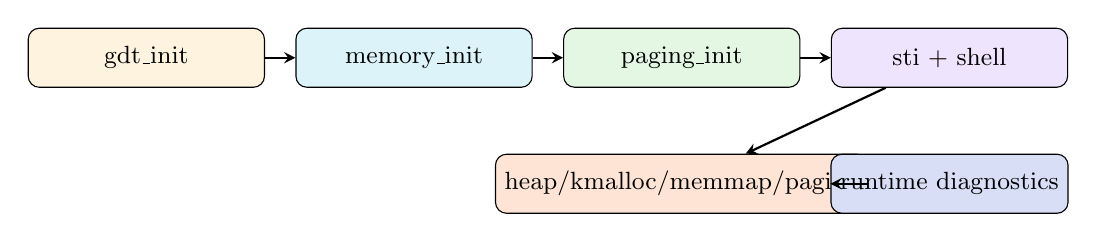
\begin{tikzpicture}[
  box/.style={rectangle,draw,rounded corners=4pt,
    minimum width=3.0cm,minimum height=0.75cm,
    align=center,font=\small},
  arr/.style={->,thick,>=stealth}]

  \node[box,fill=codeyellow!40] (boot) at (0,0) {gdt\_init};
  \node[box,fill=codeblue!30] (mem) at (3.4,0) {memory\_init};
  \node[box,fill=codegreen!30] (page) at (6.8,0) {paging\_init};
  \node[box,fill=codepurple!30] (irq) at (10.2,0) {sti + shell};

  \node[box,fill=codeorange!35] (cmd) at (6.8,-1.6) {heap/kmalloc/memmap/paging};
  \node[box,fill=codewhite!80] (view) at (10.2,-1.6) {runtime diagnostics};

  \draw[arr] (boot) -- (mem);
  \draw[arr] (mem) -- (page);
  \draw[arr] (page) -- (irq);
  \draw[arr] (irq) -- (cmd);
  \draw[arr] (cmd) -- (view);
\end{tikzpicture}
\end{center}
\end{frame}

\begin{frame}[fragile]{Heap + \texttt{kmalloc} design}
\begin{lstlisting}[style=clang]
#define KERNEL_HEAP_SIZE (128 * 1024)

void memory_init() {
    uint32_t kernel_end = (uint32_t)&_kernel_end;
    heap_start_addr = align_up(kernel_end, 16);
    heap_end_addr = heap_start_addr + KERNEL_HEAP_SIZE;
    heap_curr_addr = heap_start_addr;
}

void* kmalloc(uint32_t size) {
    size = align_up(size, 8);
    if (heap_curr_addr + size > heap_end_addr) return 0;
    void* result = (void*)heap_curr_addr;
    heap_curr_addr += size;
    return result;
}
\end{lstlisting}
\end{frame}

\begin{frame}{Keyword glossary: heap terms}
  \small
  \begin{tabular}{@{}p{2.9cm}p{9.1cm}@{}}
    \toprule
    \textbf{Keyword} & \textbf{Meaning} \\
    \midrule
    \texttt{heap} & Dynamic allocation region used after kernel boot. \\
    \texttt{bump allocator} & Allocation strategy that only moves pointer forward. \\
    \texttt{kmalloc} & Kernel allocator function returning dynamic memory addresses. \\
    \texttt{alignment} & Rounding addresses/sizes to boundaries (8 or 16 bytes). \\
    \texttt{OOM} & Out of memory; allocator returns null pointer. \\
    \texttt{\_kernel\_end} & Linker symbol marking end of loaded kernel image. \\
    \bottomrule
  \end{tabular}
\end{frame}

\begin{frame}[fragile]{Memory map reporting}
\begin{lstlisting}[style=clang]
out_regions[i++] = {"IVT+BDA", 0x00000000, 0x00000500};
out_regions[i++] = {"Bootloader", 0x00007C00, 0x00007E00};
out_regions[i++] = {"Kernel image", kernel_start, kernel_end};
out_regions[i++] = {"Kernel heap", heap_start, heap_end};
out_regions[i++] = {"Kernel stack", 0x0008F000, 0x00090000};
out_regions[i++] = {"VGA text", 0x000B8000, 0x000B9000};
\end{lstlisting}
\concept{Purpose}{
  Gives immediate visibility of major memory regions from shell command \texttt{memmap}.
}
\end{frame}

\begin{frame}[fragile]{Paging implementation (optional but sexy)}
\begin{lstlisting}[style=clang]
for (int i = 0; i < 1024; i++) page_directory[i] = 0x00000002;
for (int i = 0; i < 1024; i++) first_page_table[i] = (i * 0x1000) | 0x3;

page_directory[0] = ((uint32_t)first_page_table) | 0x3;
mov page_directory -> CR3
set CR0.PG bit
\end{lstlisting}
\textbf{Result:}
\begin{itemize}
  \item Enables paging with identity mapping for first 4MB
  \item Keeps current kernel addresses valid while introducing page translation
\end{itemize}
\end{frame}

\begin{frame}{Keyword glossary: paging terms}
  \small
  \begin{tabular}{@{}p{2.9cm}p{9.1cm}@{}}
    \toprule
    \textbf{Keyword} & \textbf{Meaning} \\
    \midrule
    \texttt{paging} & CPU memory translation from virtual to physical addresses. \\
    \texttt{page directory} & Top-level table of page table pointers. \\
    \texttt{page table} & Maps virtual pages to physical frames. \\
    \texttt{identity mapping} & Virtual address equals physical address. \\
    \texttt{CR3} & CPU register storing page-directory physical base. \\
    \texttt{CR0.PG} & Control bit enabling paging mechanism. \\
    \bottomrule
  \end{tabular}
\end{frame}

\begin{frame}{Shell commands added for this stage}
  \begin{itemize}
    \item Memory core: \texttt{heap}, \texttt{kmalloc N}, \texttt{memmap}, \texttt{paging}
    \item Time/date: \texttt{time}, \texttt{set time HH:MM:SS}, \texttt{calendar}
    \item Utility: \texttt{echo TEXT}, \texttt{reboot} (plus existing commands)
  \end{itemize}
  \concept{Why shell mattered}{
    We turned memory internals into observable runtime behavior without external debugger tooling.
  }
\end{frame}

\begin{frame}{Changes to pre-existing modules}
  \small
  \begin{tabular}{@{}p{2.5cm}p{9.5cm}@{}}
    \toprule
    \textbf{Module} & \textbf{Change} \\
    \midrule
    \texttt{kernel.c} & Added \texttt{memory\_init()} and \texttt{paging\_init()} before interrupt enable. \\
    \texttt{shell.c} & Added memory/time/calendar/paging command handlers and parser logic. \\
    \texttt{printk.c} & Added \texttt{print\_hex()} for address and flag reporting. \\
    \texttt{linker.ld} & Exported \texttt{\_kernel\_start}/\texttt{\_kernel\_end} symbols. \\
    \texttt{Makefile} & Added compile/link rules for \texttt{memory}, \texttt{paging}, and \texttt{rtc} modules. \\
    \texttt{bootloader.asm} & Expanded kernel read path to safely load larger intermediate kernel image. \\
    \bottomrule
  \end{tabular}
\end{frame}

\begin{frame}{Validation checklist for Chapter 6}
  \begin{enumerate}
    \item Boot and reach prompt without resets
    \item Run \texttt{heap} and verify used/free counters
    \item Run \texttt{kmalloc 64} repeatedly and observe address progression
    \item Run \texttt{memmap} and verify kernel/heap/stack/VGA ranges
    \item Run \texttt{paging} and verify enabled state
    \item Run \texttt{time} and \texttt{calendar} to test RTC path
  \end{enumerate}
\end{frame}

\begin{frame}{What is still next (advanced kernel memory)}
  \begin{itemize}
    \item Freeing allocator: \texttt{kfree()} and free-list or slab-like strategy
    \item Page-fault handler and demand mapping
    \item Virtual memory manager beyond first 4MB identity map
    \item Physical frame allocator backed by BIOS/E820 memory discovery
  \end{itemize}
  \warn{Current stage is correct as "intermediate kernel", not final memory subsystem.}
\end{frame}

\begin{frame}{Outcome}
  \begin{itemize}
    \item MyOS now has a real memory-management baseline
    \item Shell can introspect and exercise core memory features live
    \item Paging is enabled and integrated in boot path
    \item Platform is ready for process model and advanced VM work
  \end{itemize}
  \vspace{8pt}
  \begin{center}
    \Large \textbf{Chapter 6 completes the intermediate memory milestone.}
  \end{center}
\end{frame}

\end{document}
